\section{Lucky Patcher} \label{section:luckypatcher-explain}
On its official website, Lucky Patcher is described as "[...] a great Android tool to remove ads, modify apps permissions, backup and restore apps, bypass premium applications license verification, and more" \cite{luckyPatcherOfficial}.
It is written by a developer calling himself ChelpuS and currently on version is 6.0.7 (03/03/2016).
\newline
Lucky Patcher offers different modifications which can be used to alter functions of an application.
They can be applied to remove the license verification in premium apps or Google Ads and to change or restrict permissions and activities \cite{luckyPatcherOfficial}.
\newline
\gls{luckypatcherg} requires no technical knowledge and offers automatic cracking for non professionals.
This combination makes it a popular and an effective tool with a high potential for creating damage. \cite{munteanLicense}
\newline
\begin{figure}[h]
    \centering
    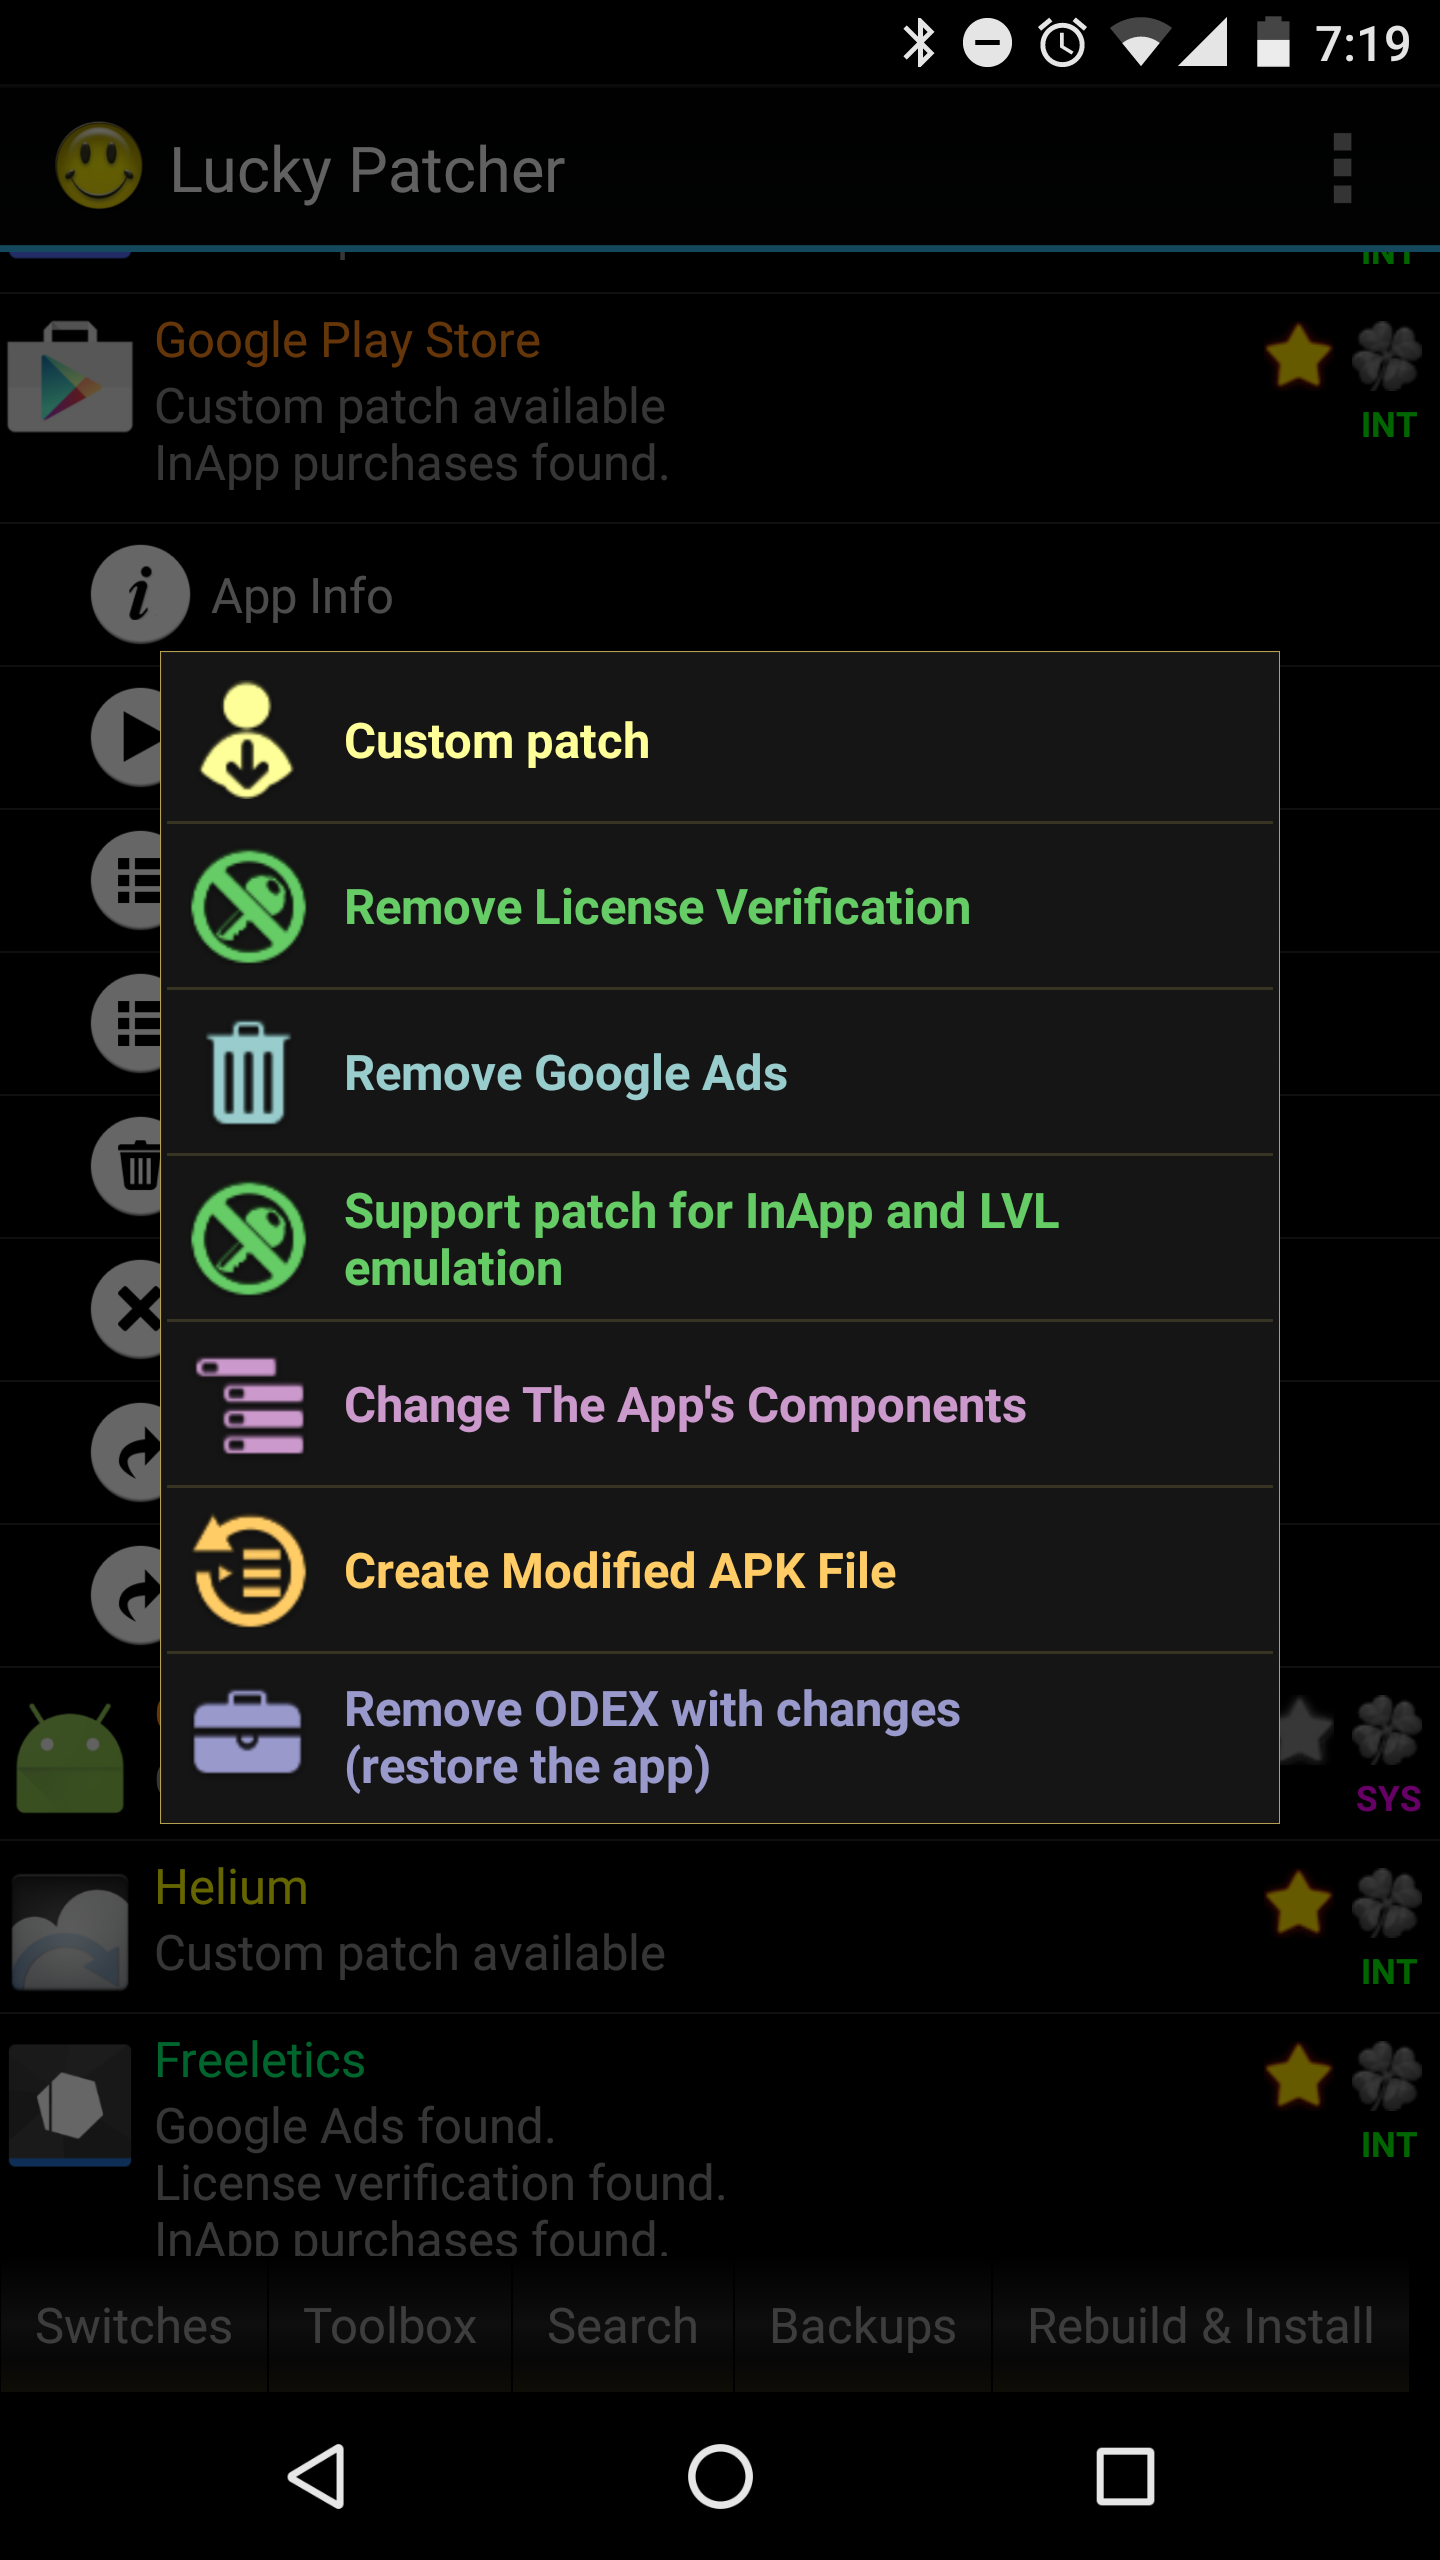
\includegraphics[width=0.3\textwidth]{data/luckyFeatures.png}
    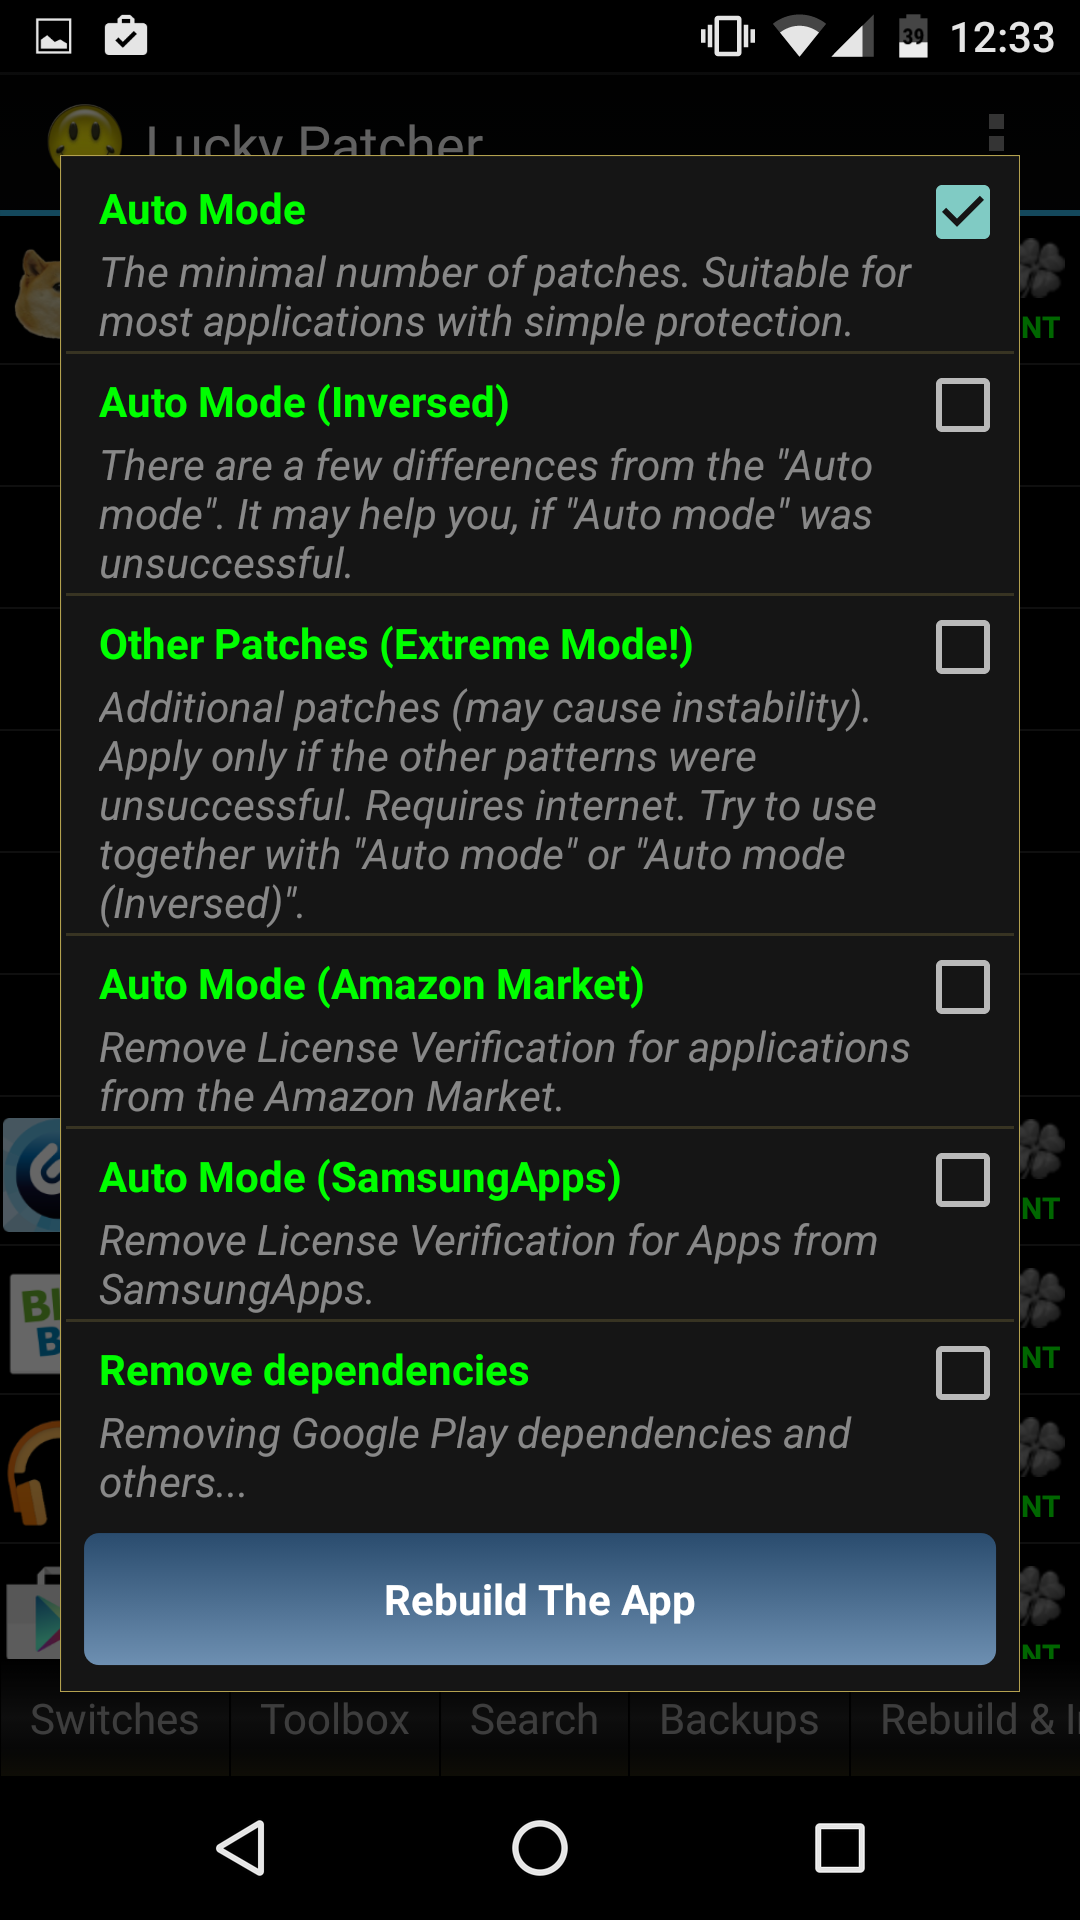
\includegraphics[width=0.3\textwidth]{data/luckyModi.png}
    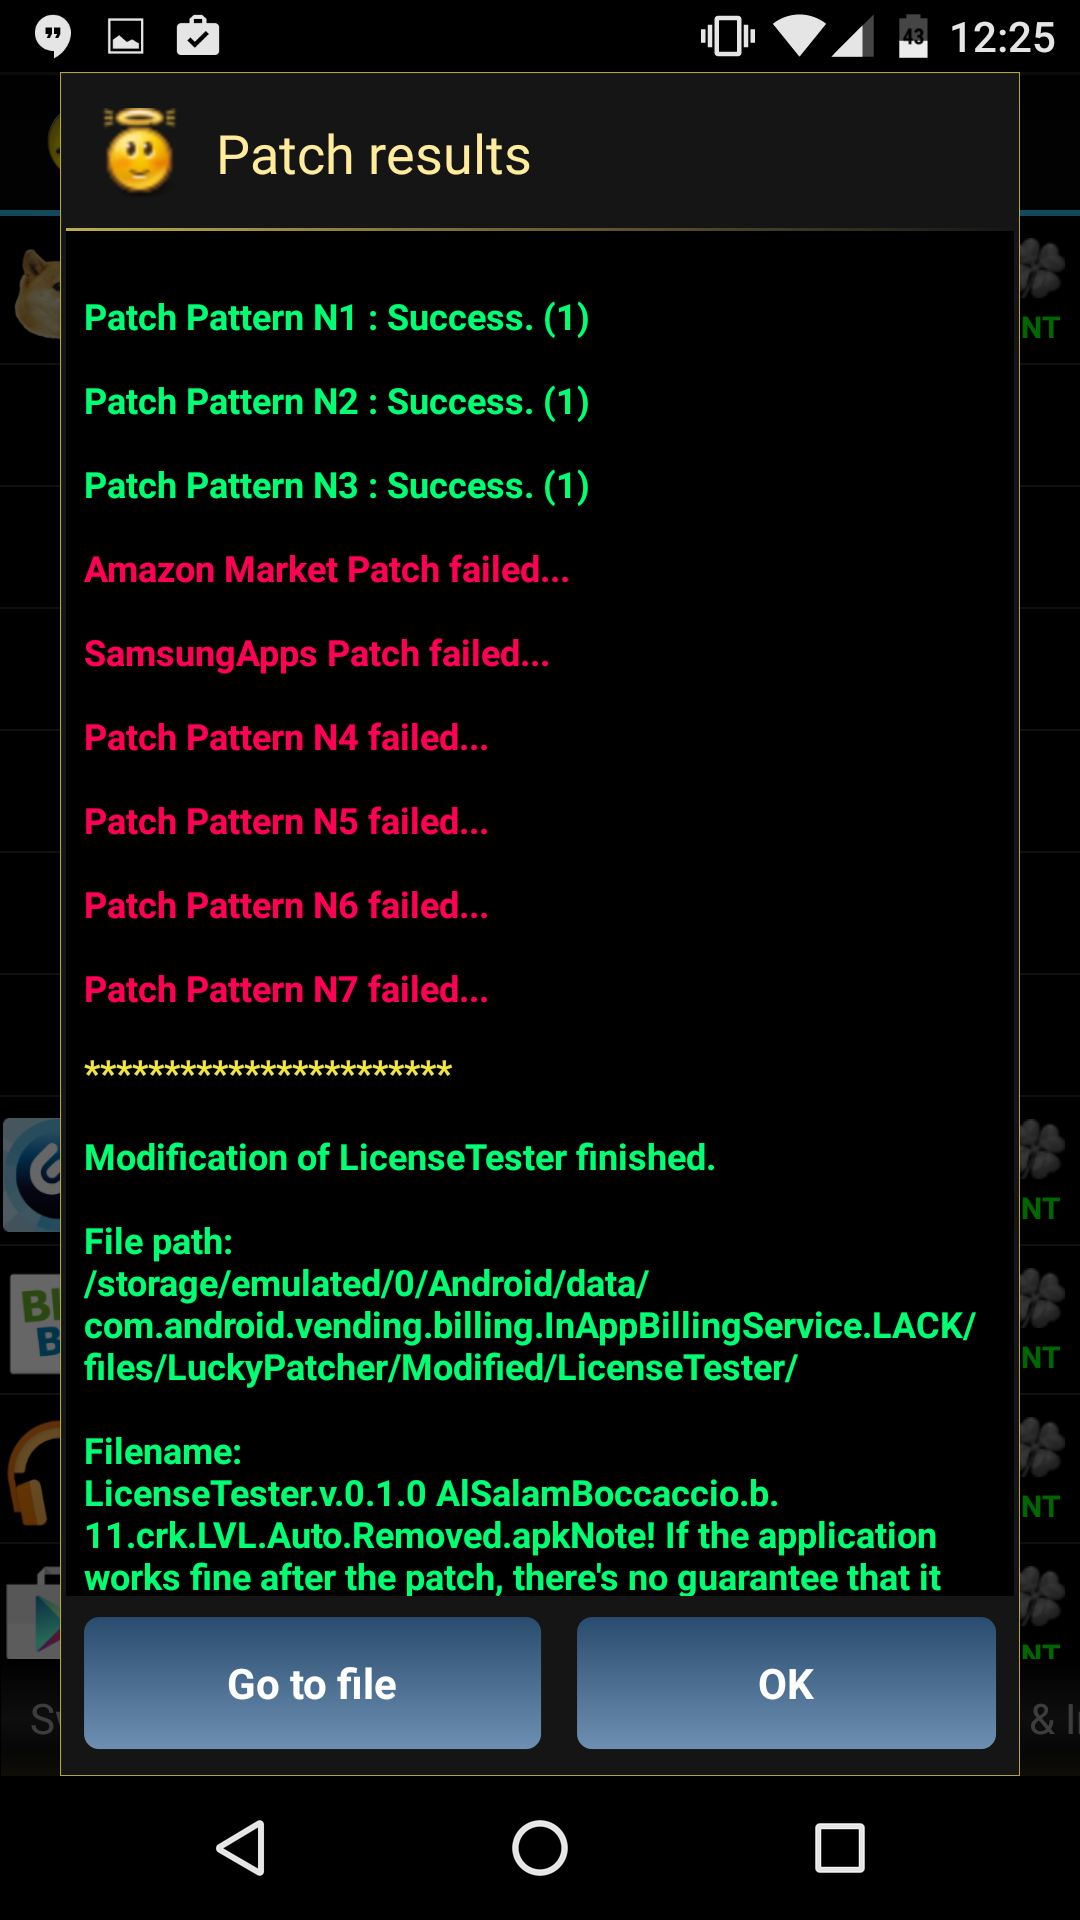
\includegraphics[width=0.3\textwidth]{data/luckyPatching.png}
    \caption{Left to right: Features offered LuckyPatcher, modes to crack license verification and the result after patching}
    \label{fig:luckyScreen}
\end{figure}
The application can be downloaded as an \gls{apk} from the official website \cite{luckyPatcherOfficial} and installed on any device, \textit{root} is not required.
After the launch of \gls{luckypatcherg}, all installed applications are shown in a list.
A colored text indicates what patches are available and can be applied to an application.
In order to unlock all features of \gls{luckypatcherg}, the device has to be rooted.
\newline
When an application is selected, a submenu offers various actions, e.g. to get information about the app or run it.
The patches menu opens the submenu of figure~\ref{fig:luckyScreen}, on the left.
It shows the available patches for this application.
\newline
There are two types of patches.
The first type is the \textit{custom patch} and the second type are universal patches.
Their goal is the disabling of the license verification libraries, removing Google Ads and rebuilding of the application to use the emulated \gls{lvl} and in-app billing \gls{api}.
\newline
\gls{luckypatcherg} offers two different approaches to apply these patches.
The first approach is to apply them directly on the device and requires \textit{root}.
This method creates an \gls{odex} version of the patched application in the Dalvik cache on the device.
The second approach is the creation of a modified \gls{apk}.
The same patches as in the first approach are available after selection, but they are not applied directly on the phone.
This approach extracts the application of choice from the storage, applies the selected modifications and creates a new \gls{apk}.
This cracked application can either be installed on the device after removing the original \gls{apk} or transferred to another device.
\newline
The custom patch is the most powerful modification.
It applies changes specifically designed for the chosen application.
The custom patches have to be provided by users who reverse engineered the application and created a solution which can be applied with \gls{luckypatcherg}.
The changes are either applied by replacing the original \textit{*.so} file of the native library with a cracked one or by injecting a bytecode sequence into the application, disabling the desired feature.
\newline
\newline
This thesis focuses on the \textit{Auto Modes} \gls{luckypatcherg} provides for voiding the implementation of the license verification libraries.
The goal of circumventing the license check is to make the pirated application work as if it had been legally acquired from a corresponding store.
\newline
There are six automatic modes available as seen in figure~\ref{fig:luckyScreen} in the middle.
Their description is rather short and does not offer information of how the modes are applied and working.
\newline
The patching starts when a mode is selected.
When the process is finished, a result screen is shown as seen in figure~\ref{fig:luckyScreen} on the right.
It is indicated that different patching patterns are used to void the license verification.
The different patching patterns are analysed and explained in section~\ref{section:luckypatcher-patterns}.
/newline
Lucky Patcher does neither guarantee that all license verification related restrictions are removed nor that the application works at all.
\newline
\newline
As described in section~\ref{section:lvl}, the license verification is implemented as client-server connection.
The server communication is secure against man in the middle attacks or spoofing, as messages are encrypted \cite{munteanLicense}.
\gls{luckypatcherg} is taking a different path by modifying the application itself.
A black box analysis is made to identify what the strategy targets and alters.
